\documentclass[11pt]{article}
\usepackage[margin=1in]{geometry}
\usepackage{amsfonts, amsmath, amssymb}
\usepackage[none]{hyphenat}
\usepackage{fancyhdr}
\setlength{\headheight}{13.6pt}
\usepackage{graphicx}
\usepackage{float}
\usepackage[nottoc, notlot, notlof]{tocbibind}
\usepackage{url}

\pagestyle{fancy}
\fancyhead{}
\fancyfoot{}
\fancyhead[L]{\slshape \MakeUppercase{Place Title Here}}
\fancyhead[R]{\slshape Student Name}
\fancyfoot[C]{\thepage}
%\renewcommand{\headrulewidth}{0pt}
\renewcommand{\footrulewidth}{0pt}

\parindent 0ex
%\setlength{\parindent}{4em}
%\setlength{\parskip}{1em}
\renewcommand{\baselinestretch}{1.5}

\begin{document}

\begin{titlepage}
\begin{center}
\vspace*{1cm}
\Large{\textbf{IB Mathematics SL}}\\
\Large{\textbf{Internal Assessment}}\\
\vfill
\line(1,0){400}\\[1mm]
\huge{\textbf{This is a Sample Title}}\\[3mm]
\Large{\textbf{- This is a Sample Subtitle -}}\\[1mm]
\line(1,0){400}\\
\vfill
By Student Name\\
Candidate \# \\
\today
\end{center}
\end{titlepage}

\tableofcontents
\thispagestyle{empty}
\clearpage

\section{Introduction}

The internally assessed component in these courses is a mathematical exploration. 
This is a short report written by the student based on a topic chosen by him or her, 
and it should focus on the mathematics of that particular area. The emphasis is on 
mathematical communication (including formulae, diagrams, graphs and so on), with 
accompanying commentary, good mathematical writing and thoughtful reflection. 
A student should develop his or her own focus, with the teacher providing feedback 
via, for example, discussion and interview. This will allow all students to develop an 
area of interest for them, without a time constraint as in an examination, and will allow 
all to experience a feeling of success. \cite{DBHS1}

In addition to testing the objectives of the courses, the exploration is intended to provide 
students with opportunities to increase their understanding of mathematical concepts and 
processes, and to develop a wider appreciation of mathematics. These are noted in the aims 
of the courses, in particular aims 6–9 (applications, technology, moral, social and ethical 
implications, and the international dimension). It is intended that, by doing the exploration, 
students benefit from the mathematical activities undertaken and find them both stimulating 
and rewarding. It will enable students to acquire the attributes of the \textbf{IB} learner profile.\footnote{An example footnote}

\section{Scoring Criteria}

\subsection{Communication}

This criterion assesses the organization and coherence of the exploration. 
A well-organized exploration includes an introduction, has a rationale 
(which includes explaining why this topic was chosen), describes the aim 
of the exploration and has a conclusion. A coherent exploration is logically 
developed and easy to follow. Graphs, tables and diagrams should accompany 
the work in the appropriate place and not be attached as appendices to the document.

\subsection{Mathematical Presentation}

This criterion assesses to what extent the student is able to use appropriate 
mathematical language (notation, symbols, terminology), define key terms where 
required, and use multiple forms of mathematical representation such as formulae, 
diagrams, tables (see table \ref{tab:data1}), charts, graphs and models, where appropriate.

\begin{table}[H]
    \centering
    \begin{tabular}{|c|c|c|c|} \hline
        $x$ & 0 & 1 & 2 \\ \hline
        $f(x)$ & 3 & 6 & 9 \\ \hline
    \end{tabular}
    \caption{Caption goes here}
    \label{tab:data1}
\end{table}

Students are expected to use mathematical language when communicating 
mathematical ideas, reasoning and findings, where appropriate. Students 
are encouraged to choose and use appropriate \textbf{ICT} tools such as 
graphic display calculators, \textbf{screenshots}, graphing (see figure \ref{fig:squeeze}), spreadsheets, 
databases, drawing and word-processing software, as appropriate, to 
enhance mathematical communication.

\begin{figure}[H]
    \centering
    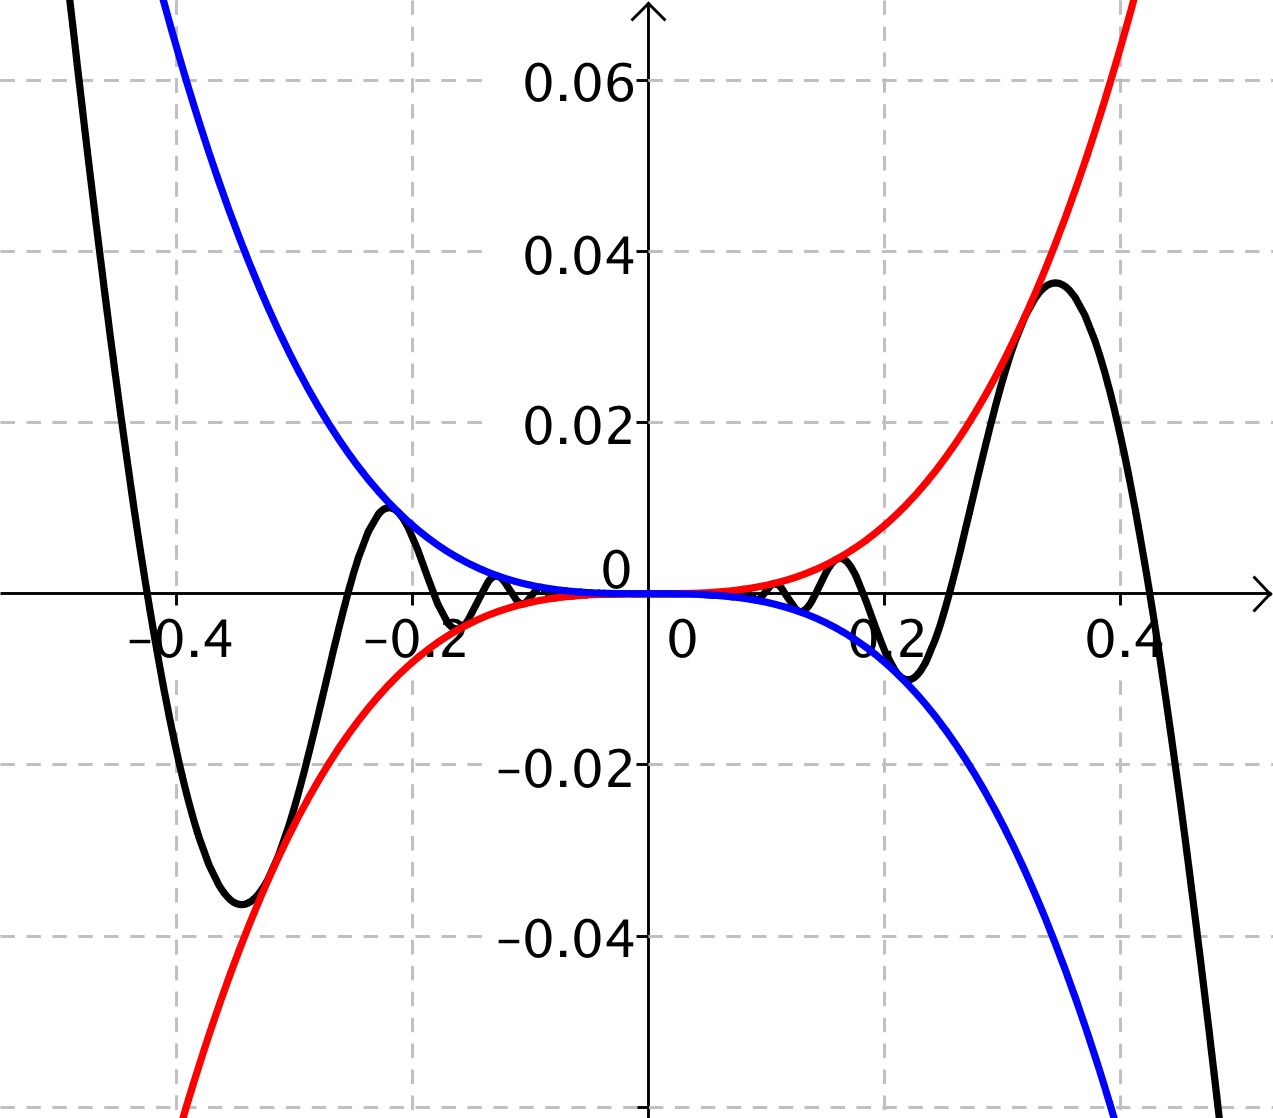
\includegraphics[scale=0.5]{limit}
    \caption{The Squeeze Theorem}
    \label{fig:squeeze}
\end{figure}

\subsection{Personal Engagement}

This criterion assesses the extent to which the student engages with the 
exploration and makes it their own. Personal engagement may be recognized 
in different attributes and skills. These include thinking independently and/or 
creatively, addressing personal interest and presenting mathematical ideas in 
their own way.

To receive full marks, students must show evidence of outstanding personal 
engagement. The work should be original. It may be from historical ideas and 
real world situations (for example, socio–economic, political awareness). 
Students should create some examples or present some ideas explained in depth.

\subsection{Reflection}

This criterion assesses how the student reviews, analyses and evaluates the 
exploration. Although reflection may be seen in the conclusion to the exploration, 
it may also be found throughout the exploration.

Students should ideally have continuous reflection throughout the task, which 
should include the following: identify and address issues as the piece develops, 
discuss limitations of the work where applicable, provide ideas for extensions, 
and reflect on the significance of the findings.

\subsection{Use of Mathematics}

This criterion assesses to what extent and how well students use mathematics 
in the exploration. Students are expected to produce work that is commensurate 
with the level of the course. The mathematics explored should either be part of 
the syllabus, or at a similar level or beyond. It should not be completely based 
on mathematics listed in the prior learning. If the level of mathematics is not 
commensurate with the level of the course, a maximum of two marks can be 
awarded for this criterion.

The mathematics can be regarded as correct even if there are occasional minor 
errors as long as they do not detract from the flow of the mathematics or lead 
to an unreasonable outcome. Sophistication in mathematics may include 
understanding and use of challenging mathematical concepts, looking at a 
problem from different perspectives and seeing underlying structures to link 
different areas of mathematics. Rigour involves clarity of logic and language 
when making mathematical arguments and calculations. Precise mathematics 
is error-free and uses an appropriate level of accuracy at all times.

\section{Conclusion}

The exploration is intended to be an opportunity for students to use mathematics 
to develop an area of interest to them rather than merely to solve a problem set 
by someone else. Criterion C (personal engagement) will be looking at how well 
the student is able to demonstrate that he or she has ``made the 
exploration their own'' and expressed ideas in an individual way.

It is difficult to be prescriptive about mathematical writing. However, the 
Mathematics \textbf{SL} guide and the Mathematics \textbf{HL} guide state that 
6–12 pages should be appropriate. A common failing of mathematical writing is 
excessive repetition, and this should be avoided, as such explorations will be 
penalized for lack of conciseness. However, it is recognized that some 
explorations will require the use of several diagrams, which may extend them 
beyond the page limit.

\section{Using \LaTeX{}}

Be sure to cite any sources you use throughout the text. 
There are more advanced methods of creating bibliographies, 
but the method used here is simplest for a short list of references.

Also note that you may have to compile the document twice 
before you see updated citations and the updated table of contents.

\pagebreak
\begin{thebibliography}{}

\bibitem{DBHS1}
Alcosser, Howard.  
``Diamond Bar High School.''  
\textit{Internal Assessment: Mathematical Exploration}.  
Web. 27 May 2015.

\bibitem{DBHS2}
Alcosser, Howard.  
``Diamond Bar High School.''  
\textit{Mathematical Exploration Rubric}.  
Web. 27 May 2015.  
\url{http://dbhs.wvusd.k12.ca.us/ourpages/auto/2010/10/1/38060822/IA_2014_rubric.pdf}.

\bibitem{name1}
Lastname, Firstname.  
\textit{Title of Book},  
City of Publication:  
Publisher,  
Year of Publication.  
Medium of Publication.

\bibitem{name2}
Author(s).  
``Title of Article.''  
Title of Periodical  
Day Month Year:  
pages.  
Medium of publication.

\bibitem{name3}
Author(s).  
``Title of Article.''  
Title of Journal  
Volume.Issue (Year):  
pages.  
Medium of publication.

\bibitem{name4}
Editor, author, or compiler name (if available).  
\textit{Name of Site.}  
Name of institution or organization affiliated with the site (sponsor or publisher),  
date of resource creation (if available).  
Medium of publication.  
Date of access.  
\url{http://www.samplewebsite.com}.

\bibitem{name5}
Artist's name,  
\textit{The Work of Art},  
Date of creation,  
Institution and city where the work is housed.  
\textit{Name of Website},  
Medium of publication,  
Date of access.

\end{thebibliography}

\end{document}
